\section{Benefits of Tiny Tasks}
\label{sec:benefits}
Tiny tasks benefit data center workloads by providing inherent elasticity:
fine-grained units of work can be dynamically allocated to machines as
resources become available, eliminating stragglers and issues of data skew,
and allowing jobs to use available resources without sacrificing fairness
when new jobs are submitted.

\subsection{Handling of skew and stragglers}
Parallel workloads can suffer from outlier tasks that run for much longer than the median task length and dominate jobs' run times.
Outliers can be caused by uneven divisions of work across tasks (skew) or by conditions on particular machines (stragglers).


Tiny tasks avoid both causes of outliers.
In general, increasing the number of tasks results in a more even partitioning of records across tasks, avoiding skew due to uneven partitioning.
By splitting the total work into more tasks, faster machines can perform a greater share of the work because less work is queued in tasks on slow machines.
This mitigates the effects of expensive records and adapts to heterogeneous clusters composed of fast and slow machines.

Figure~\ref{fig:binpacked} demonstrates the improvement if we
achieved perfect load-balancing across tasks by assigning individual records to tasks.
\fixme{Describe the data source for Figure~\ref{fig:binpacked}.}
Assigning tiny tasks to idle machines at run-time approximates a static bin-packing of work across machines, but does not require accurate cost-estimation.

\begin{figure}[t]
\centering
\hspace{2ex}
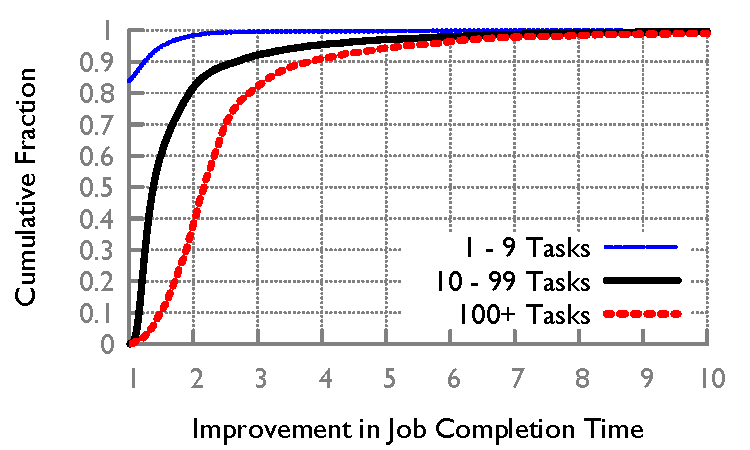
\includegraphics[width=0.5\textwidth]{figures/binpacked1-sep}
\vspace{-4ex}
\caption{Ideal improvement from binpacking tasks.}
\vspace{-2ex}
\label{fig:binpacked}
\end{figure}



\subsection{Fairness NEED A BETTER NAME}
Diagram here showing a before and after of what happens when a new job arrives
(and another job was already using the entire cluster)

Talk about Amoeba tradeoff.

Big win here is the ability seamlessly integrate batch and interactive workloads.

Simulation of response times for differently sized jobs as paralleism increases.

